\documentclass[../linalg.tex]{subfiles}
\graphicspath{{\subfix{../figures/}}}
\begin{document}
\chapter{Linear Equations in Linear Algebra}
\section{Systems of Linear Equations}
A linear equation in the variables $x_1,\dots,x_n$ is an equation that can be written in the form 
\[ a_1x_1+a_2x_2+\dots + a_nx_n=b\]
where $b$ and the coefficients $a_1,\dots,a_n$ are real or complex numbers, usually known in advance.

A system of linear equations (or a linear system) is a collection of one or more linear equations involving the same variables - say, $x_1,\dots,x_n$.

A solution of the system is a list ($s_1,s_2,\dots,s_n$) of numbers that makes each equation a true statement when the values $s_1,\dots,s_n$ are substituted for $x_1,\dots,x_n$, respectively.

The set of all possible solutions is called the solution set of a linear system.

Two linear systems are called equivalent if they have the same solution set.

A system of linear equations has 
\begin{enumerate}
    \item no solution, or
    \item exactly one solution, or
    \item infinitely many solutions.
\end{enumerate}

A system of linear equations is said to be consistent if it has either one solution or infinitely many solutions.

A system is inconsistent if it has no solution.

The essential information of a linear system can be recorded compactly in a rectangular array called a matrix. Given a system,
\begin{align*}
    x_1-2x_2+x_3=0\\
    2x_2-8x_3=8\\
    -4x_1+5x_2+9x_3=-9
\end{align*}, with the coefficients of each variable aligned in columns, the matrix 
\[ \begin{bmatrix}
    1&-2&1\\ 0&2&-8\\ -4&5&9
\end{bmatrix} \]
is called the coefficient matrix (or matrix of coefficients) of the system.

An augmented matrix of a system consists of the coefficient matrix with an added column containing the constants from the right sides of the equations.

For the given system of equations,
\[ \begin{bmatrix}
    1&-2&1&0\\ 0&2&-8&8\\ -4&5&9&-9
\end{bmatrix} \]
is called the augmented matrix of the system.

The size of a matrix tells how many rows and columns it has. If $m$ and $n$ are positive integers, an $m\times n$ matrix is a rectangular array of numbers with $m$ rows and $n$ columns. (The number of rows always comes first.)

For example, $\begin{bmatrix}
    1&2&3&4\\ 5&6&7&8
\end{bmatrix}$ is a $2\times 4$ matrix.

The basic strategy for solving a linear system is to replace one system with an equivalent system (i.e., one with the same solution set) that is easier to solve.

Elementary row operations include the following:
\begin{enumerate}
    \item (Replacement) Replace one row by the sum of itself and a multiple of another row. For example, $2R_1+R_3 \rightarrow R_3$.
    \item (Interchange) Interchange two rows. For example: $R_1\leftrightarrow R_4$.
    \item (Scaling) Multiply all entries in a row by a nonzero constant. For example: $\frac{1}{3}R_3\rightarrow R_3$.
\end{enumerate}

Two matrices are called row equivalent if there is a sequence of elementary row operations that transforms one matrix into the other.

It is important to note that row operations are reversible.

If the augmented matrices of two linear systems are row equivalent, then the two systems have the same solution set.

Two fundamental equations about a linear system are as follos:
\begin{enumerate}
    \item Is the system consistent: that is, does at least one solution exist?
    \item If a solution exists, is it the only one, that is, is it unique?
\end{enumerate}

\begin{example}
    Determine if the following system is consistent:
    \begin{align*}
        x_2-4x_3=8\\
        2x_1-3x_2+2x_3=1\\
        5x_1-8x_2+7x_3=1
    \end{align*}

    First interchange row 1 and 2 to get \[\begin{bmatrix}
        2 & -3 & 2 & 1\\
        0 & 1 & -4 & 8\\
        5 & -8 & 7 & 1
    \end{bmatrix}\]

    Do the operation $-\frac{5}{2}R_1+R_3\rightarrow R_3$:
    \[\begin{bmatrix}
        2 & -3 & 2 & 1\\
        0 & 1 & -4 & 8\\
        0 & -\frac{1}{2} & 2 & -\frac{3}{2}
    \end{bmatrix}\] 

    Do the operation $2R_3+R_2\rightarrow R_3$:
    \[\begin{bmatrix}
        2 & -3 & 2 & 1\\
        0 & 1 & -4 & 8\\
        0 & 0 & 0 & 5
    \end{bmatrix}\]

    That bottom row says that no $x_1,x_2$ or $x_3$ will equal 5, or $0=5$. This is not true, so the system is inconsistent.
\end{example}

\section{Row Reduction and Echelon Forms}
In the definitions that follow, a nonzero row or column in a matrix means a row or column that contains at least one nonzero entry; a leading entry of a row refers to the leftmost nonzero entry (in a nonzero row).

A rectangular matrix is in echelon form (or row echelon form) if it has the following three properties:
\begin{enumerate}
    \item All nonzero rows are above any rows of all zeros.
    \item Each leading entry of a row is in a column to the right of the leading entry of the row above it.
    \item All entries in a column below a leading entry are zeros.
\end{enumerate}

If a matrix in echelon form satisfies the following additional conditions, then it is in reduced echelon form (or reduced row echelon form):
\begin{enumerate}
    \item The leading entry in each nonzero row is $1$.
    \item Each leading $1$ is the only nonzero entry in its column.
\end{enumerate}

An echelon matrix (respectively, reduced echelon matrix) is one that is in echelon form (respectively, reduced echelon form.)

Any nonzero matrix may be row reduced (i.e., transformed by elementary row operations) into more than one matrix in echelon form, using different sequences of row operations. However, the reduced echelon form one obtains from a matrix is unique.

\begin{theorem}[Uniqueness of the Reduced Echelon Form]
    Each matrix is row equivalent to one and only one reduced echelon matrix.
\end{theorem}

If a matrix $A$ is row equivalent to an echelon matrix $U$, we call $U$ an echelon form (or row echelon form) of $A$; if $U$ is in reduced echelon form, we call $U$ the reduced echelon form of $A$.

A pivot position in a matrix $A$ is a location in $A$ that corresponds to a leading $1$ in the reduced echelon form of $A$. A pivot column is a column of $A$ that contains a pivot position.

\begin{example}
    Row reduce the matrix $A$ below to echelon form, and locate the pivot columns of $A$.
    \[ \begin{bmatrix}
        0 & -3 & -6 & 4 & 9\\
        -1 & -2 & -1 & 3 & 1\\
        -2 & -3 & 0 & 3 &-1\\
        1&4&5&-9&-7
    \end{bmatrix} \]

    The following row operations will give the matrix:
    \begin{itemize}
        \item $R_1 \leftrightarrow R_4$
        \item $R_1 + R_2 \rightarrow R_2$ and $2R_1+R_3\rightarrow R_3$
        \item $\frac{1}{2}R_2\rightarrow R_2$ and $\frac{1}{5}R_3 \rightarrow R_3$
        \item $-R_2+R_3\rightarrow R_3$ and $3R_2+R_4\rightarrow R_4$
        \item $R_3\leftrightarrow R_4$
    \end{itemize}

    The resulting matrix is $\begin{bmatrix}
        1 & 4 & 5 & -9 & -7\\
        0 & 1 & 2 & -3 & -3\\
        0 & 0 & 0 & -8 & 0\\
        0 & 0 & 0 & 0 & 0
    \end{bmatrix}$
\end{example}

Row Reduction Algorithm:

Step 1: Begin with the leftmost nonzero column. This is a pivot column. The pivot position is at the top.

Step 2: Select a nonzero entry in the pivot column as a pivot. If necessary, interchange rows to move this entry into the pivot position.

Step 3: Use row replacement operations to create zeros in all positions below the pivot.

Step 4: Cover (or ignore) the row containing the pivot position and cover all rows, if any, above it. Apply steps 1-3 to the submatrix that remains. Repeat the process until there are no more nonzero rows to modify. 

Step 5: Beginning with the rightmost pivot and working upward and to the left, create zeros above each pivot. If a pivot is not $1$, make it $1$ by a scaling operation.

The combination of steps 1-4 is called the forward phase of the row reducing algorithm. Step 5, which produces the unique reduced echelon form, is called the backward phase.

\begin{example}
    Apply elementary row operations to transform the following matrix first into echelon form and then into reduced echelon form.

    Do the following row operations:
    \begin{itemize}
        \item $R_1\leftrightarrow R_3$
        \item $-R_1+R_2\rightarrow R_2$
        \item $\frac{1}{2}R_2\rightarrow R_2$
        \item $-3R_2+R_3\rightarrow R_3$
        \item $-6R_3+R_1\rightarrow R_1$ and $-R_3+R_2\rightarrow R_2$
        \item $9R_2+R_1\rightarrow R_1$
        \item $\frac{1}{3}R_1\rightarrow R_1$
    \end{itemize}
    
    The matrix that results is $\begin{bmatrix}
        1&0&-2&3&0&-24\\
        0&1&-2&2&0&-7\\
        0&0&0&0&1&4
    \end{bmatrix}$
\end{example}

The row reduction algorithm leads to an explicit description of the solution set of a linear system when the algorithm is applied to the augmented matrix of the system.

Suppose, for example, the augmented matrix of a linear system has been changed into the equivalent reduced echelon form.
\[ \begin{bmatrix}
    1&0&-5&1\\
    0&1&1&4\\
    0&0&0&0
\end{bmatrix}\]

The variables $x_1$ and $x_2$ corresponding to pivot columns in the matrix are called basic variables. The other variable, $x_3$ is called a free variable.

\begin{theorem}[Existence and Uniqueness Theorem]
    A linear system is consistent if and only if the rightmost column of the augmented matrix is not a pivot column - i.e., if and only if an echelon form of the augmented matrix has no row of the form 
    \begin{center}
        $\begin{bmatrix}
            0&\dots & 0 & b
        \end{bmatrix}$ with $b$ nonzero.
    \end{center}
    If a linear system is consistent, then the solution set contains either (i) a unique solution, when there are no free variables, or (ii) infinitely many solutions, when there is at least one free variable.
\end{theorem}

\section{Vector Equations}
Vectors in $\mathbb{R}^2$:
\begin{itemize}
    \item A matrix with only one column is called a column vector, or simply a vector.
    \item An example of a vector with two entries is
    \[ W = \begin{bmatrix}
        w_1\\w_2
    \end{bmatrix}\]
    where $w_1$ and $w_2$ are any real numbers.
    \item The set of all vectors with two entries is denoted by $\mathbb{R}^2$ (read ``$r$-two'')
\end{itemize}

\begin{itemize}
    \item The $\mathbb{R}$ stands for the real numbers that appear as entries in the vector, and the exponent $2$ indicates that each vector contains two entries.
    \item Two vectors in $\mathbb{R}^2$ are equal if and only f their corresponding entries are equal.
    \item Given two vectors $\vec{u}$ and $\vec{v}$ in $\mathbb{R}^2$, their sum is the vector $\vec{u}+\vec{v}$ obtained by adding corresponding entries of $\vec{u}$ and $\vec{v}$.
    \item Given a vector $\vec{u}$ and a real number $c$, the scalar multiple of $\vec{u}$ by $c$ is the vector $c\vec{u}$ obtained by multiplying each entry in $\vec{u}$ by $c$.
\end{itemize}

\begin{example}
    Given $u=\begin{bmatrix}
        1\\-2
    \end{bmatrix}$ and $v=\begin{bmatrix}
        2\\-5
    \end{bmatrix}$, find 

    (a) $4\vec{u}$

    $4\vec{u}=4\begin{bmatrix}
        1\\-2
    \end{bmatrix}=\begin{bmatrix}
        4\\-8
    \end{bmatrix}$

    (b) $(-3)\vec{v}$

    $(-3)\begin{bmatrix}
        2\\-5
    \end{bmatrix}=\begin{bmatrix}
        -6\\15
    \end{bmatrix}$

    (c) $4\vec{u}+(-3)\vec{v}$

    $\begin{bmatrix}
        4\\-8
    \end{bmatrix}+\begin{bmatrix}
        -6\\15
    \end{bmatrix}=\begin{bmatrix}
        -2&7
    \end{bmatrix}$
\end{example}

\begin{itemize}
    \item Consider a rectangular coordinate system in the plane. Because each point in the plane is determined by an ordered pair of numbers, we can identify a geometric point $(a,b)$ with the column vector $\begin{bmatrix}
        a\\b
    \end{bmatrix}$
    \item So we may regard $\mathbb{R}^2$ as the set of all points in the plane.
\end{itemize}

If $\vec{u}$ and $\vec{v}$ in $\mathbb{R}^2$ are represented as points in the plane, then $\vec{u}+\vec{v}$ corresponds to the fourth vertex of the parallelogram whose other vertices are $\vec{u}, \vec{0}$ and $\vec{v}$.
\begin{center}
    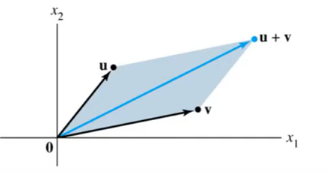
\includegraphics[width=0.4\textwidth]{1.1.PNG}
\end{center}

\begin{itemize}
    \item Vectors in $\mathbb{R}^3$ are $3\times 1$ column matrices with three entries.
    \item They are represented geometrically by points in a three-dimensional coordinate space, with arrows from the origin sometimes included for visual clarity.
    \item If $n$ is a positive integer, $\mathbb{R}^n$ (read ``$r$-$n$'') denotes the collection of all lists (or ordered $n$-tuples) of $n$ real numbers, usually written as $n\times 1$ column matrices, such as 
\end{itemize}
\[ u = \begin{bmatrix}
    u_1 \\ u_2 \\ \vdots \\ u_n
\end{bmatrix}\]

The vector whose entries are all zero is called the zero vector and is denoted by $\vec{0}$.

For all $\vec{u}$, $\vec{v}$, $\vec{w}$ in $\mathbb{R}^n$ and all scalars $c$ and $d$:
\begin{enumerate}
    \item $\vec{u}+\vec{v}=\vec{v}+\vec{u}$
    \item $(\vec{u}+\vec{v})+\vec{w}=\vec{u}+(\vec{v}+\vec{w})$
    \item $\vec{u}+\vec{0}=\vec{0}+\vec{u}=\vec{u}$
    \item $\vec{u}+(-\vec{u})=-\vec{u}+\vec{u}=\vec{0}$, where $-\vec{u}$ denotes $(-1)\vec{u}$
    \item $c(\vec{u}+\vec{v})=c\vec{u}+c\vec{v}$
    \item $(c+d)\vec{u}=c\vec{u}+d\vec{u}$
    \item $c(d\vec{u})=(cd)(\vec{u})$
    \item $1\vec{u}=\vec{u}$
\end{enumerate}

Given vectors $\vec{v_1}, \vec{v_2},\dots,\vec{v_p}$ in $\mathbb{R}^n$ and given scalars $c_1, c_2,\dots,c_p$, the vector $\vec{y}$ is defined by 
\[ \vec{y}=c_1\vec{v_1}+\dots +c_p\vec{v_p}\]
is called a linear combination of $\vec{v_1},\dots,\vec{v_p}$ with weights $c_1,\dots,c_p$.

The weights in a linear combination can be any real numbers, including zero.

\begin{example}
    Let $a_1=\begin{bmatrix}
        1\\-2\\-5
    \end{bmatrix}, a_2=\begin{bmatrix}
        2\\5\\6
    \end{bmatrix}$ and $b=\begin{bmatrix}
        7\\4\\-3
    \end{bmatrix}$. Determine whether $\vec{b}$ can be generated (or written) as a linear combination of $\vec{a_1}$ and $\vec{a_2}$. That is, determine whether weights $x_1$ and $x_2$ exist such that 
    \[ x_1a_1 + x_2a_2 = b \]

    Using matrix operations, we get that $x_1\begin{bmatrix}
        -1\\-2\\-5
    \end{bmatrix}+x_2\begin{bmatrix}
        2\\5\\6
    \end{bmatrix}=\begin{bmatrix}
        7\\4\\-3
    \end{bmatrix}$

    This is written as $\begin{bmatrix}
        x_1\\-2x_1\\-5x_1
    \end{bmatrix}+\begin{bmatrix}
        2x_2\\5x_2\\6x_2
    \end{bmatrix}=\begin{bmatrix}
        7\\4\\3
    \end{bmatrix}$.

    This can be written as a system of equations.

    \begin{align*}
        x_1+2x_2=7\\
        -2x_1+5x_2=4\\
        -5x_1+6x_2=-3
    \end{align*}

    Using the following row operations:
    \begin{itemize}
        \item $2R_1+R_2 \rightarrow R_2$ and $5R_1+R_3\rightarrow R_3$
        \item $\frac{1}{9}R_2 \rightarrow R_2$ and $\frac{1}{12}R_3\rightarrow R_3$
        \item $-2R_2 + R_1 \rightarrow R_1$ and $-R_2+R_3 \rightarrow R_3$
    \end{itemize}

    We get $x_1=3$ and $x_2=2$.

    So we can write $b=3a_1+2a_2$.
\end{example}

\begin{definition}
    If $\vec{v_1},\dots,\vec{v_p}$ are in $\mathbb{R}^n$, then the set of all linear combinations of $\vec{v_1},\dots,\vec{v_p}$ is denoted by Span$\{\vec{v_1},\dots,\vec{v_p}\}$ and is called the subset of $\mathbb{R}^n$ spanned (or generated) by $\vec{v_1},\dots,\vec{v_p}$. That is, Span$\{\vec{v_1},\dots,\vec{v_p}\}$ is the collection of all vectors that can be written in the form 
    \[ c_1 v_1+c_2 v_2+\dots+c_p v_p\]
    with $c_1,\dots, c_p$ scalars.
\end{definition}

Let $\vec{v}$ be a nonzero vector in $\mathbb{R}^3$. Then Span$\{\vec{v}\}$ is the set of all scalar multiples of $\vec{v}$, which is the set of points on the line in $\mathbb{R}^3$ through $\vec{v}$ and $\vec{0}$.

If $\vec{u}$ and $\vec{v}$ are nonzero vectors in $\mathbb{R}^3$, with $\vec{v}$ not a multiple of $\vec{u}$, then Span$\{\vec{u},\vec{v}\}$ is the plane in $\mathbb{R}^3$ that contains $\vec{u},\vec{v}$, and $\vec{0}$. In particular, Span$\{\vec{u},\vec{v}\}$ contains the line in $\mathbb{R}^3$ through $\vec{u}$ and $\vec{0}$ and the line through $\vec{v}$ and $\vec{0}$.

\section{The Matrix Equation Ax = b}
\section{Solution Sets of Linear Systems}
\section{Applications of Linear Systems}
\section{Linear Independence}
\section{Introduction to Linear Transformations}
\section{The Matrix of a Linear Transformation}
\section{Linear Models in Business, Science, and Engineering}
\end{document}